% Couverture Thèse TPT Latex v2
% Fabrice Linot 04/12/11 

\documentclass[11pt,a4paper]{book}
\usepackage[left=1.3cm,top=0cm,right=1.3cm,bottom=1.2cm]{geometry}
\usepackage{graphicx}
\usepackage{eso-pic}
\usepackage{array}
\usepackage[french]{babel}
\usepackage[utf8x]{inputenc}
\usepackage[T1]{fontenc}
\usepackage{textcomp}
\usepackage{helvet}	% or \usepackage{lmodern}
\renewcommand\textnumero{n$^{\textsf{{\tiny O}}}$}
\renewcommand{\familydefault}{\sfdefault}

\usepackage{ifpdf}
\newcommand\BackgroundPic{
\ifpdf
	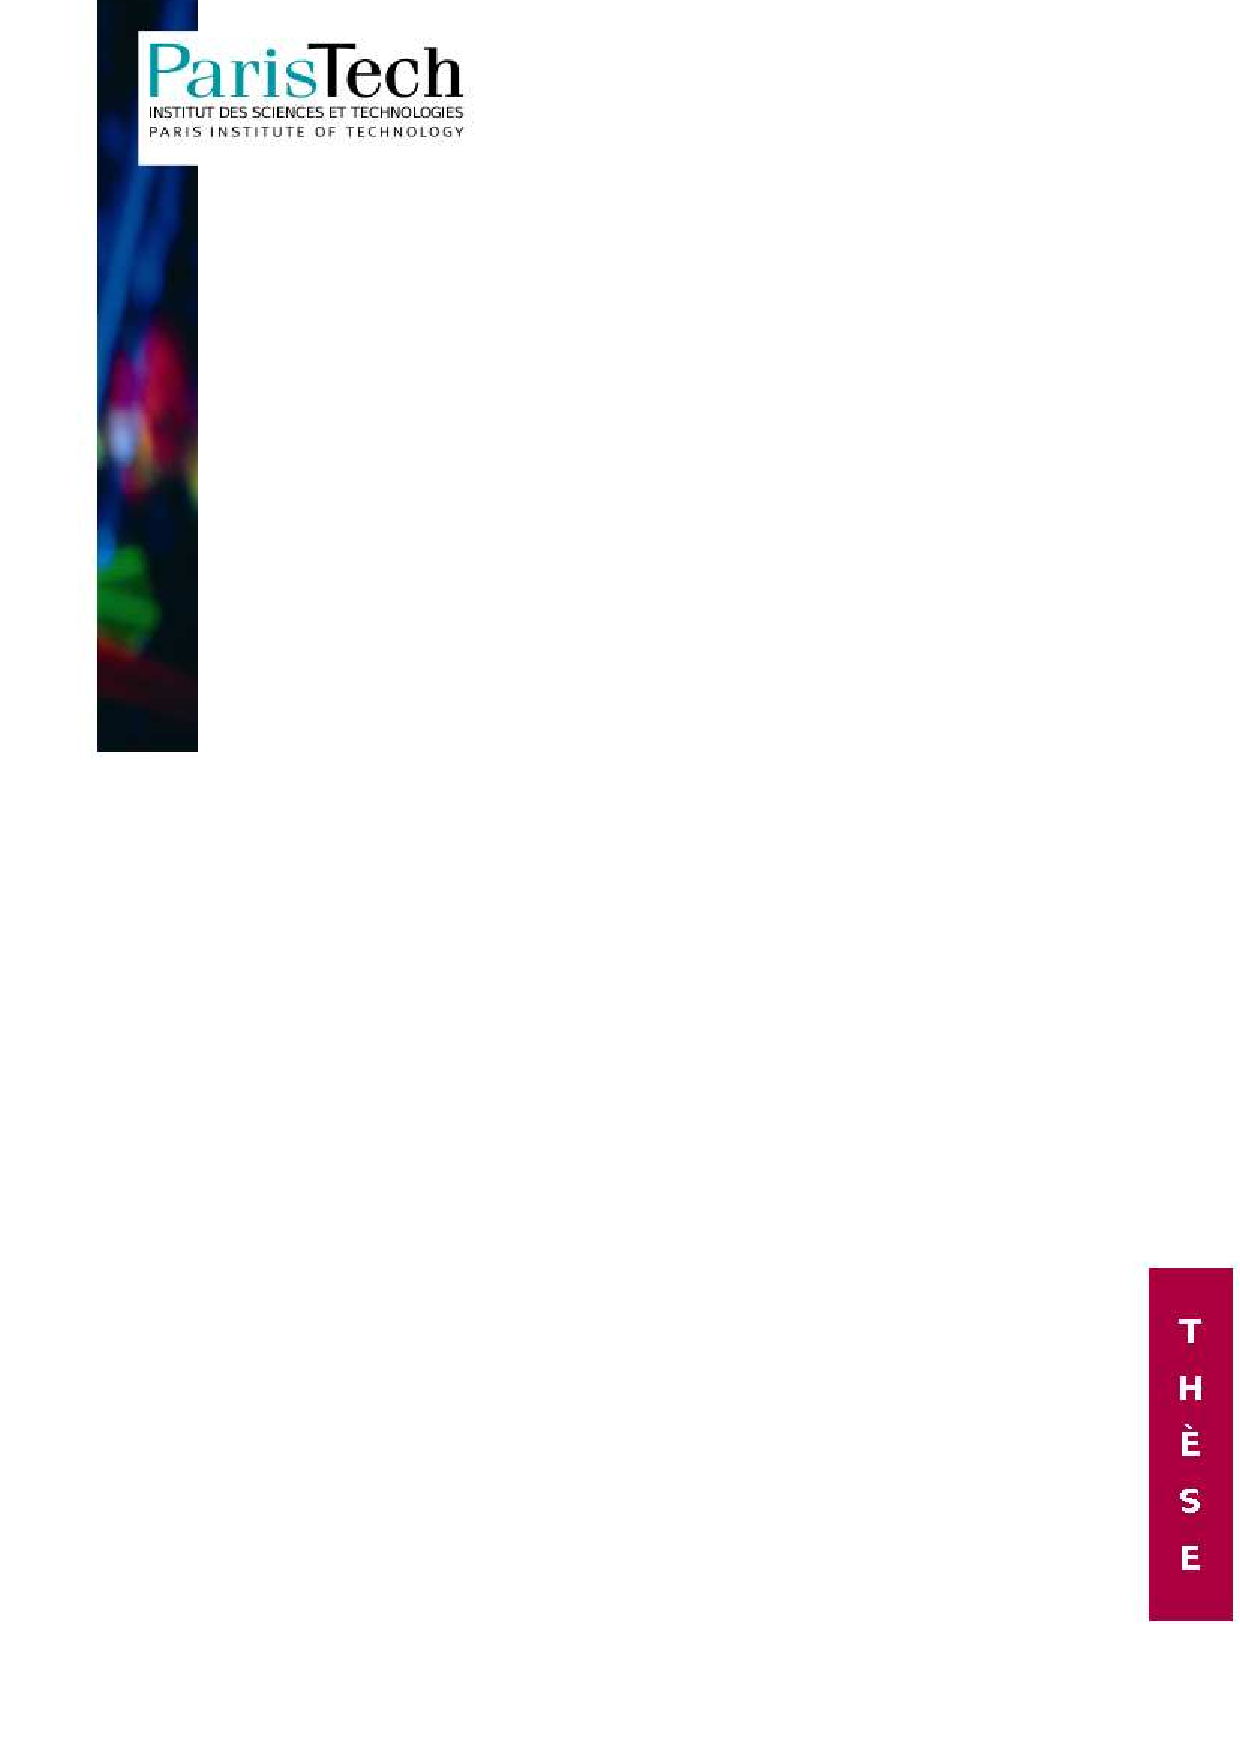
\includegraphics[height=\paperheight,width=\paperwidth]{BackgroundTPT_Premiere.pdf}
\else
	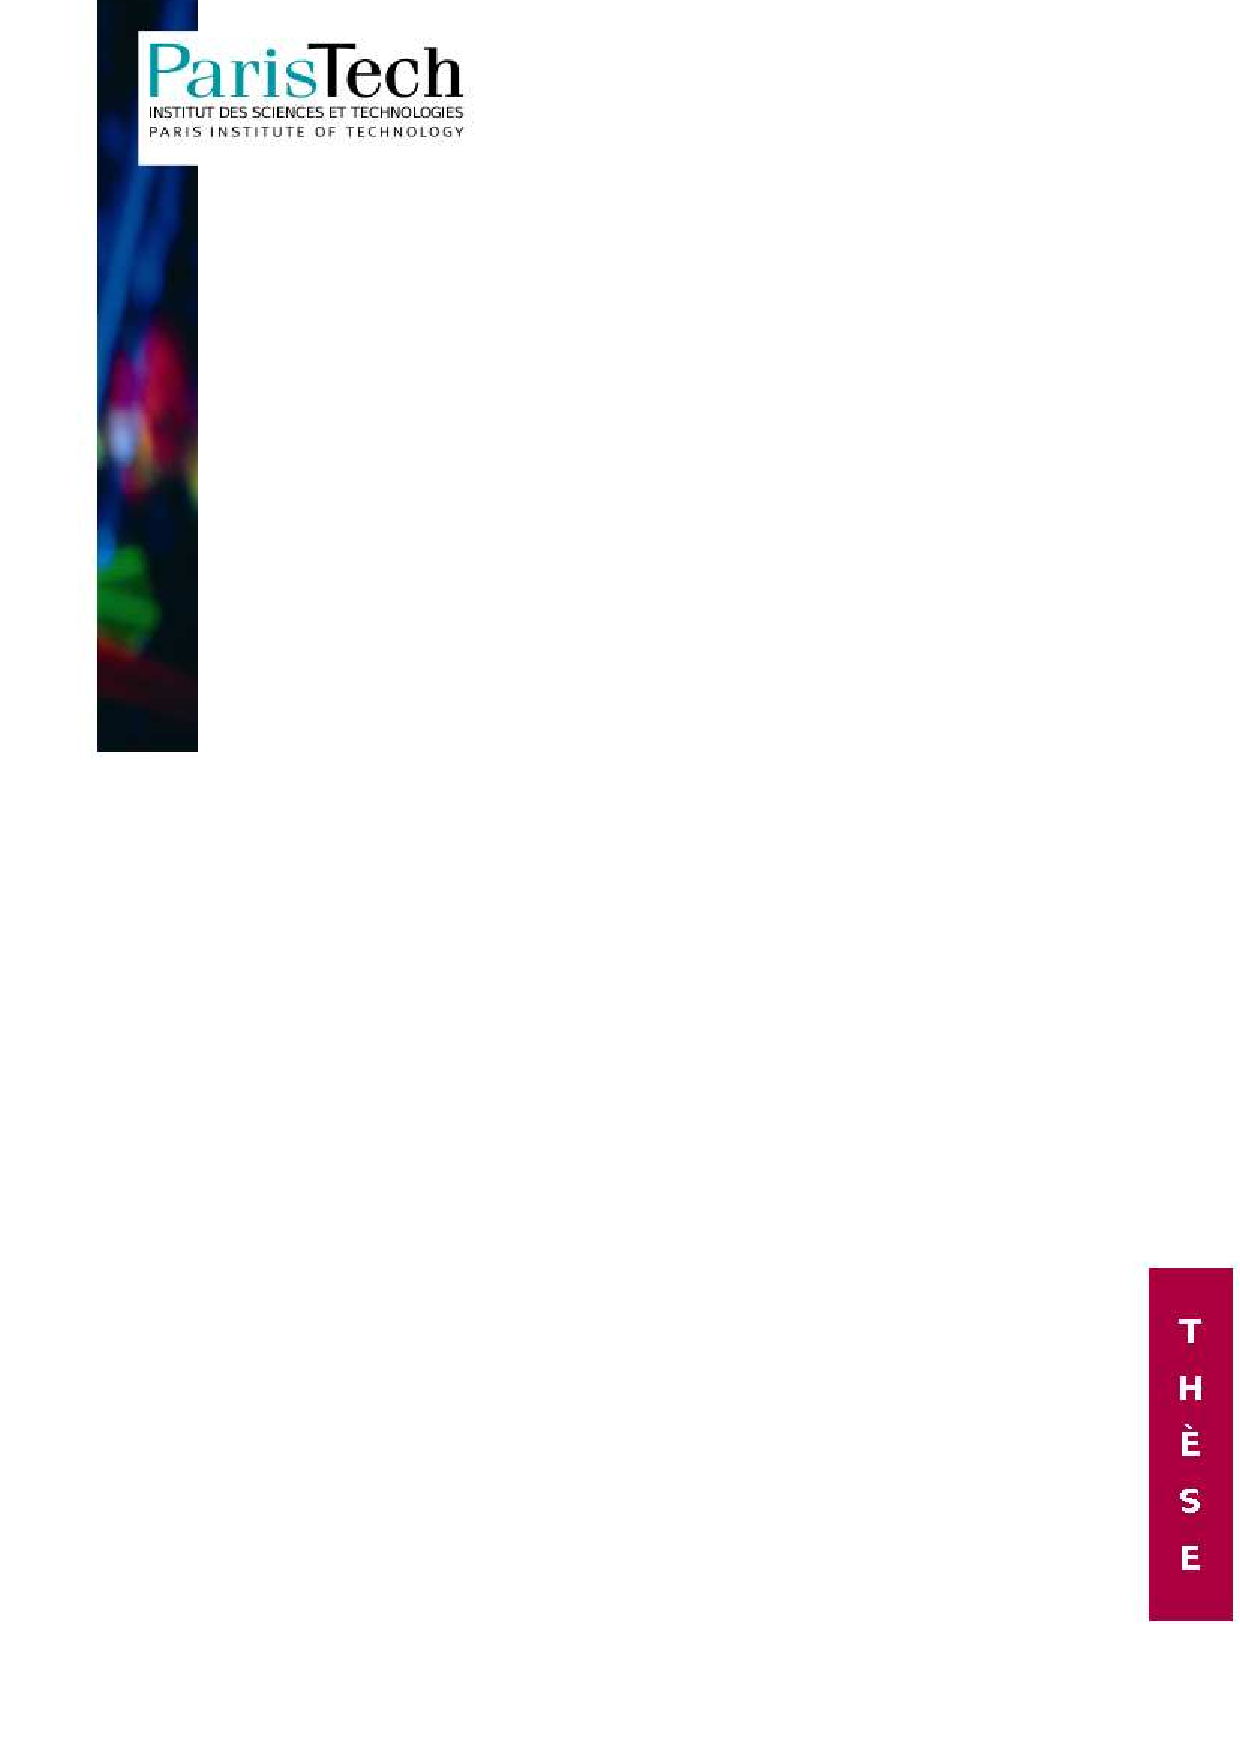
\includegraphics[height=\paperheight,width=\paperwidth]{BackgroundTPT_Premiere.pdf}
\fi
}

\pagestyle{empty}

\begin{document}
\AddToShipoutPicture*{\BackgroundPic}
~


\begin{flushright}


\includegraphics[scale=0.45]{logo_TPT.pdf}

{\small {2015-EURECOM-00xx~~~~}}
\end{flushright}



%\vspace{0.cm}
\begin{center}
%



\includegraphics[scale=0.65]{logo_edite.pdf} \\
{\small {EDITE - ED 130}}


%
\vspace{.5cm}
%
%
%
%{\Large École doctorale \textnumero XX: texte}\\		% version une ligne
%{\Large École doctorale \textnumero XX:\\ texte}\\		% version deux lignes (changer les espaces en conséquence
%
%
%
\vspace{1.0cm}
%
%
%
{\LARGE {\bf Doctorat ParisTech}}\\
\vspace{1.1cm}
{\LARGE {\bf T H È S E}}\\
\vspace{0.5cm}
{\normalsize {\bf pour obtenir le grade de docteur délivré par}}\\
%
%
%
\vspace{.9cm}
%
%
%
%
{\LARGE {\bf TELECOM ParisTech}}\\
\vspace{0.6cm}
{\Large {\bf Spécialité \og Informatique \fg}}\\
%
%
%
\vspace{.8cm}
%
%
%
{\normalsize {\it présentée et soutenue publiquement par}}\\
\vspace{0.7cm}
{\Large {\bf Ghislain Auguste ATEMEZING}}\\
\vspace{0.24cm}
{\normalsize le 10 avril 2015}\\
%
%
%
\vfill
%
%
%
\textcolor[RGB]{191,18,56}{
\noindent
{\LARGE {\bf Publishing and Consuming Geo-Spatial and \\[.6cm]Government Data on the Semantic Web}}\\
}
%
%Publishing and Consuming Geo-Spatial and Government Data on the Semantic Web
%
\vfill~\vfill
%
%
%
{\normalsize
\begin{tabular}{c}
Directeur de thèse:					{\bf Raphaël TRONCY}\\
%Co-encadrement de la thèse:		{\bf Prénom NOM}
\end{tabular}
}
\end{center}
%
%
%
\vfill
%
%
%
\flushleft
\begin{minipage}{.9\textwidth}	% ou .91\textwidth si vous n'avez pas assez de place
{\bf Jury}\\
% Mme/M. Prénom NOM, Titre, Unité de recherche, Ecole 
{\bf M. Sören AUER}, {\small Professeur, IAIS, Université de Bonn, Allemagne}
	\hfill Rapporteur\\
{\bf Mme. Chantal REYNAUD}, {\small Professeur, INRIA Saclay, Université de Paris XI, France}
	\hfill Rapporteur\\
{\bf M. Roberto GARCIA}, {\small Maître de Conférences associé, Universitat de Lleida, Espagne }
	\hfill Examinateur\\
{\bf M. Andreas HARTH}, {\small Maître de Conférences, Institut AIFB, Karlsruhe, Allemagne}
	\hfill Examinateur\\
{\bf Mme. Elisabeth METAIS}, {\small Professeur, CNAM - Equipe ISID, France}
	\hfill Examinateur\\
{\bf M. Sébastien MUSTIERE}, {\small HDR, COGIT-IGN, France}
	\hfill Invité\\
%{\bf Mme/M. Prénom NOM}, {\small Titre, Unité de recherche, Ecole}
%	\hfill Fonction\\
%{\bf Mme/M. Prénom NOM}, {\small Titre, Unité de recherche, Ecole}
%	\hfill Fonction\\

\end{minipage}\\
%
%
%
%\vspace{-.3cm}
%
%
%
\centering
{\bf TELECOM ParisTech}\\
{\small école de l'Institut Télécom - membre de ParisTech}
%
%
%
\end{document}
